\chapter{LabVIEW and Arduino}
If you have covered Chapter 2 \& 3, you are more than ready to start using $\labview$ to manipulate real world objects. Although this chapter would be largely self contained, it is assumed that you have covered chapter 1 and understand the basics of $\labview$. Where relevant, you will be referred to chapter 2 or the $\labview$ helpfiles in order to aid you through examples\\

This chapter will focus on the ``LiNX'' package, it should be installed with your community edition of $\labview$. To check if you do have this package installed, go to the block diagram and open the functions palette. Near the bottom of the menu, you will see a folder called ``Hobbyist", this contains all the functions you need to talk to your Arduino board. If it is not installed, you can use the JKI package manager to install it.
\section{Getting Started}
Before we begin sending commands to our Arduino board, we need to flash specific firmware onto the little microcontroller of the board. To do this, you need the LiNX firmware wizard. You can open the firmware wizard from your taskbar by going to Tools\textrightarrow Maker Hub\textrightarrow LiNX\textrightarrow LiNX Firmware Wizard.\\

Before you move along, the rest of the chapter assumes you will be using an Arduino Uno, I have tested it on an Arduino Nano before so your mileage may vary. Since the firmware wizard does not have much in the way of troubleshooting options, you should make sure that you can flash programs onto your device using the Arduino Studio program. Make note of the serial address, you will need it for the next step.\\

Figure \ref{FirmwareTool} shows the wizard open, use the following settings: (Assuming you will be using an Arduino Uno)
\begin{itemize}
	\item \textbf{Device Family}: Arduino
	\item \textbf{Device Type}: Arduino Uno
	\item \textbf{Firmware Update Method}: Serial / USB
\end{itemize}
\begin{figure}
	\centering
	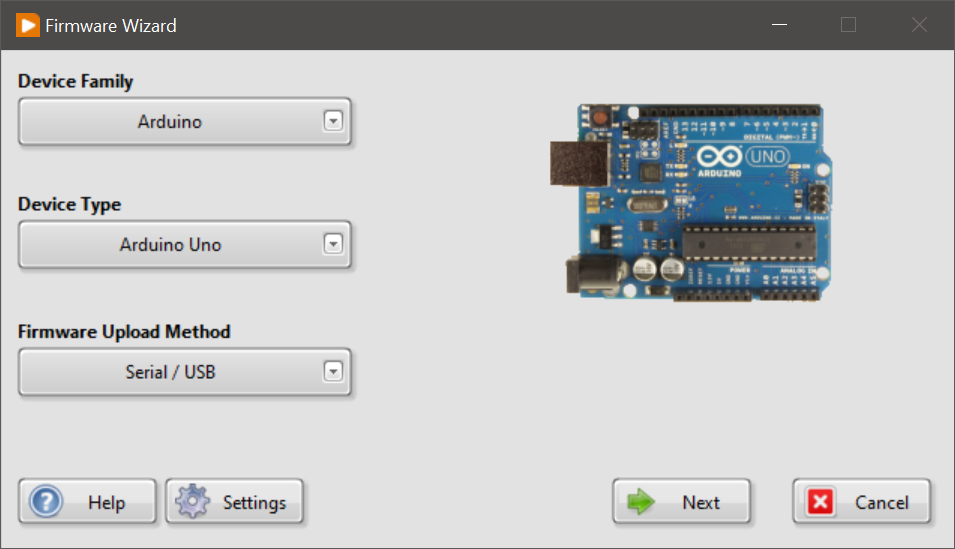
\includegraphics[width=0.75\textwidth]{FirmwareTool}
	\caption{The LiNX firmware wizard, we use this tool to make the Arduino learn $\labview$.}
	\label{FirmwareTool}
\end{figure}
Pressing next will take you to the port selection screen, make sure you select the COM port your Arduino board is connected to. If you do not see it here, make sure that you have the device plugged in and that the drivers for it is installed.\\

The last screen you should leave as is, figure \ref{FirmwareConf}, it sets the method in which the wizard flashes the microcontroller, in this case Serial/USB, and what type of firmware to install. It is possible to create your own firmware, but this beyond the scope of this book.\\
\begin{figure}
	\centering
	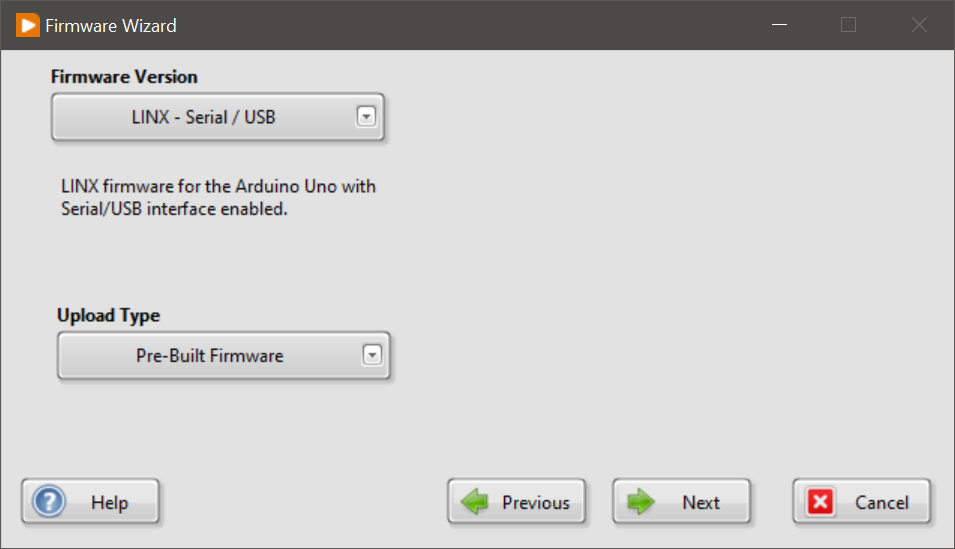
\includegraphics[width=0.75\textwidth]{FirmwarePath}
	\caption{Firmware flash settings screen, you should leave this as is.}
	\label{FirmwareConf}
\end{figure}

Once the firmware flashing is complete, a friendly window will tell you so, press the ``Launch Example'' button to test drive the new system. Figure \ref{BuiltInArduinoEg} shows the VI that opens. %TODO Add the picture please
 Here you set the COM port, like you did previously, and select the output channel to be 13. Run this VI and press the LED that says ``Click Here'', you will observe that the LED on your Arduino reflects the status of the LED in the VI. Go ahead and press it as many times as you like, you now have control over a real world object through the power of your mouse.
 
\section{Writing and Reading Ports}
We now take a small step back in time to review how Arduino code is structured. Figure \ref{ArduinoStartCode} shows the typical structure of an Arduino project. The ``setup'' block runs once, this is where \textit{you} configure all the inputs and outputs of the Arduino board and provide the code to setup a LCD display module, for example. The ``run'' loop runs continuously %TODO check naming of this loop
performing the instructions step-by-step, until the end of time, or when the power cable is unplugged.\\

Fortunately, you may use the same development patern for building code, for the Arduino, in $\labview$. There are few little extras along the way, such as opening a link to a board and managing the closing of any connections you made.\\

It is right about now where you will realise the power of $\labview$, not so much in the graphical programming style, but the amount of libraries that exist to ease the development of prototype projects.\\

\subsection{Opening a serial port to an Arduino}
\subsection{Configuring I/O}
\subsection{The main program loop} 
\subsection{Closing all connections}
\section{Quite Advanced Projects}